\documentclass[aspectratio=169,xcolor=dvipsnames,11pt]{beamer}

% The original project template uses CleanEasy. TeX Live provides the same
% theme package, so the visual system is preserved without changing themes.
\usetheme{CleanEasy}

\usepackage{fontspec}
\usepackage{amsmath,amssymb,mathtools}
\usepackage{unicode-math}
\setmainfont{Times New Roman}
\setsansfont{Times New Roman}
\setmonofont{Courier New}
\setmathfont{TeX Gyre Termes Math}
\usefonttheme{professionalfonts}
\renewcommand{\familydefault}{\rmdefault}

\usepackage{booktabs,tabularx,array}
\usepackage{siunitx}
\usepackage{graphicx}
\usepackage{tikz}
\usetikzlibrary{arrows.meta,positioning,calc,fit}
\usepackage{hyperref}
\usepackage{appendixnumberbeamer}

\graphicspath{{figures/}}
\sisetup{detect-all,round-mode=places,round-precision=3}

\definecolor{ValidGreen}{HTML}{5EB3A8}
\definecolor{SoftGreen}{HTML}{E9F6F2}
\definecolor{WarnRed}{HTML}{EC5858}
\definecolor{SoftRed}{HTML}{F9E8E8}
\definecolor{DeepNavy}{HTML}{0D2759}
\definecolor{SoftGray}{HTML}{EEF1F4}
\definecolor{MidGray}{HTML}{6B7280}

\setbeamercolor{alerted text}{fg=WarnRed}
\setbeamercolor{example text}{fg=ValidGreen!70!black}
\setbeamercolor{normal text}{fg=black,bg=white}
\setbeamercolor{structure}{fg=DeepNavy}
\setbeamertemplate{caption}{\raggedright\insertcaption\par}
\setbeamerfont{normal text}{family=\rmfamily}
\setbeamerfont{frametitle}{family=\rmfamily,size=\Large,series=\bfseries}
\setbeamerfont{title}{family=\rmfamily,size=\LARGE,series=\bfseries}
\setbeamerfont{subtitle}{family=\rmfamily,size=\normalsize}
\setbeamerfont{block title}{family=\rmfamily,size=\large,series=\bfseries}
\setbeamerfont{block body}{family=\rmfamily}

\newcommand{\src}[1]{%
  \vfill
  {\color{MidGray}\fontsize{6.5}{7.5}\selectfont Source: #1\par}
}
\newcommand{\protocolnote}[1]{%
  {\color{MidGray}\scriptsize #1}
}
\newcommand{\resultbox}[3]{%
  \begin{beamercolorbox}[rounded=true,sep=0.45em,center,wd=\linewidth]{block body}
  {\color{DeepNavy}\Large\bfseries #1}\par
  {\small #2}\par
  {\color{MidGray}\scriptsize #3}
  \end{beamercolorbox}
}
\newcommand{\compactresultbox}[3]{%
  \begin{beamercolorbox}[rounded=true,sep=0.27em,center,wd=\linewidth]{block body}
  {\color{DeepNavy}\large\bfseries #1}\par
  {\footnotesize #2}\par
  {\color{MidGray}\tiny #3}
  \end{beamercolorbox}
}

\title[Reduced PINNs]{Reduced Physics-Informed Neural Networks\\for Parametric Poisson Equations}
\subtitle{Fast surrogate predictions for repeated one-dimensional Poisson problems}
\author[Project P13]{Huiyao Chen \and Ruojia Gu \and Yutong Hou \and Yessine Jmal \and Jiayun Wang}
\institute[CentraleSupélec]{CentraleSupélec, Université Paris-Saclay\\Supervisor: Philippe Dessante, GreePs}
\date[Feb.--Jun. 2026]{Projet S6 - P13 \textperiodcentered\ February--June 2026}

\begin{document}

% Slide 1
\begin{frame}[plain]
  \begin{tikzpicture}[remember picture,overlay]
    \node[anchor=north west,inner sep=0pt]
      at ([xshift=0.65cm,yshift=-0.48cm]current page.north west)
      {
\includegraphics[trim={8bp 0bp 4bp 3bp},clip,height=0.85cm]{logo_centralesupelec.png}};
    \node[anchor=north east,inner sep=0pt]
      at ([xshift=-0.65cm,yshift=-0.48cm]current page.north east)
      {
\includegraphics[trim={10bp 11bp 10bp 12bp},clip,height=0.85cm]{logo_geeps.png}};
  \end{tikzpicture}
  \titlepage
\end{frame}

% Slide 2
\begin{frame}{The repeated-query problem}
  \begin{columns}[c,onlytextwidth]
    \begin{column}{0.34\textwidth}
      \small
      A Poisson equation can describe electric potential between two electrodes.

      \vspace{0.65em}
      When the charge distribution changes, the potential changes with it. A parameter study therefore requires many related PDE solves.

      \vspace{0.65em}
      \begin{alertblock}{Project question}
        Can previously trained PINNs be reused instead of training a new network for every parameter value?
      \end{alertblock}
    \end{column}
    \begin{column}{0.63\textwidth}
      \includegraphics[width=\linewidth]{parametric_problem.pdf}
    \end{column}
  \end{columns}
  \src{report\_PINN.pdf, Sections 1 and 3; notebooks 03--04. Curves recomputed from the stated Poisson model.}
\end{frame}

% Slide 3
\begin{frame}{Parametric Poisson equation}
  \centering
  {\Large
  \[
    -\frac{\mathrm d^2 u}{\mathrm d x^2}
      = f(x;\mu,\sigma,A)
      = A\exp\!\left[-\frac{(x-\mu)^2}{2\sigma^2}\right],
      \qquad x\in(0,1)
  \]
  \[
    u(0)=1,
    \qquad
    u(1)=0
  \]
  }
  \vspace{0.5em}
  \begin{columns}[T,onlytextwidth]
    \begin{column}{0.30\textwidth}
      \begin{block}{Position $\mu$}
        Moves the localized source through the domain.
      \end{block}
    \end{column}
    \begin{column}{0.30\textwidth}
      \begin{block}{Width $\sigma$}
        Controls how sharply the source is concentrated.
      \end{block}
    \end{column}
    \begin{column}{0.30\textwidth}
      \begin{block}{Amplitude $A$}
        Sets the strength of the source term.
      \end{block}
    \end{column}
  \end{columns}
  \src{report\_PINN.pdf, Eqs. (1)--(6); parameter values in notebooks 06--10.}
\end{frame}

% Slide 4
\begin{frame}{PINN training uses the differential equation}
  \begin{columns}[c,onlytextwidth]
    \begin{column}{0.55\textwidth}
      \[
        \widehat u_\theta(x;\lambda)\approx u(x;\lambda),
        \qquad \lambda=(\mu,\sigma,A)
      \]
      \[
        r_\theta(x;\lambda)
        =-\partial_{xx}\widehat u_\theta(x;\lambda)-f(x;\lambda)
      \]
      \[
        \mathcal L(\theta)
        =\frac{1}{N_r}\sum_{j=1}^{N_r}|r_\theta(x_j;\lambda)|^2
        +\lambda_{\mathrm{BC}}\mathcal L_{\mathrm{BC}}
      \]
      \begin{exampleblock}{What provides supervision}
        Automatic differentiation evaluates the PDE residual. Exact solutions remain separate and are used for evaluation.
      \end{exampleblock}
    \end{column}
    \begin{column}{0.40\textwidth}
      \centering
      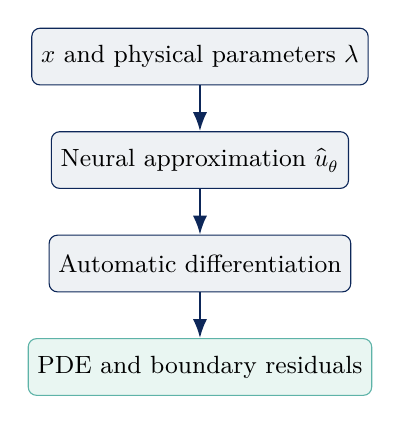
\begin{tikzpicture}[
        node distance=0.58cm,
        box/.style={draw=DeepNavy,rounded corners=3pt,fill=SoftGray,minimum width=3.2cm,minimum height=0.72cm,align=center,font=\small},
        arr/.style={-{Latex[length=2.4mm]},thick,draw=DeepNavy}
      ]
        \node[box] (input) {$x$ and physical parameters $\lambda$};
        \node[box,below=of input] (net) {Neural approximation $\widehat u_\theta$};
        \node[box,below=of net] (ad) {Automatic differentiation};
        \node[box,below=of ad,fill=SoftGreen,draw=ValidGreen] (loss) {PDE and boundary residuals};
        \draw[arr] (input)--(net);
        \draw[arr] (net)--(ad);
        \draw[arr] (ad)--(loss);
      \end{tikzpicture}
    \end{column}
  \end{columns}
  \src{report\_PINN.pdf, Section 3.4; implementations in notebooks 03--05.}
\end{frame}

% Slide 5
\begin{frame}{Hard constraints enforce both boundary values}
  \begin{columns}[c,onlytextwidth]
    \begin{column}{0.58\textwidth}
      \includegraphics[width=\linewidth]{hard_constraint.pdf}
    \end{column}
    \begin{column}{0.38\textwidth}
      {\large
      \[
        \widehat u_\theta(x)
        =1-x+x(1-x)N_\theta(x)
      \]
      }
      \vspace{0.4em}
      \begin{exampleblock}{Exact by construction}
        The correction term vanishes at $x=0$ and $x=1$, regardless of the learned network weights.
      \end{exampleblock}
      \small
      This removes the boundary penalty and lets training focus on the interior residual.
    \end{column}
  \end{columns}
  \src{report\_PINN.pdf, Eqs. (12)--(18); hard-constrained implementation in 11discrete.py.}
\end{frame}

% Slide 6
\begin{frame}{Full PINNs repeat costly optimization}
  \centering
  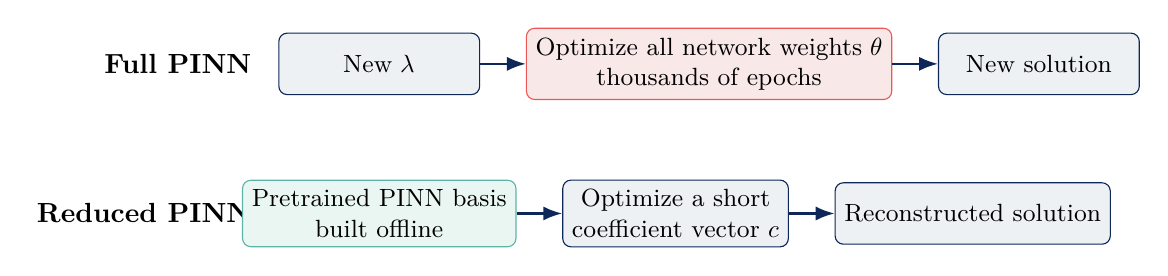
\begin{tikzpicture}[
    node distance=0.50cm and 0.58cm,
    box/.style={draw=DeepNavy,rounded corners=3pt,fill=SoftGray,minimum height=0.78cm,minimum width=2.55cm,align=center,font=\small},
    full/.style={box,fill=SoftRed,draw=WarnRed},
    reduced/.style={box,fill=SoftGreen,draw=ValidGreen},
    arr/.style={-{Latex[length=2.4mm]},thick,draw=DeepNavy}
  ]
    \node[font=\bfseries,anchor=east] (flabel) at (-5.35,1.10) {Full PINN};
    \node[box] (fquery) at (-3.85,1.10) {New $\lambda$};
    \node[full,right=of fquery] (ftrain) {Optimize all network weights $\theta$\\thousands of epochs};
    \node[box,right=of ftrain] (fout) {New solution};
    \draw[arr] (fquery)--(ftrain);
    \draw[arr] (ftrain)--(fout);

    \node[font=\bfseries,anchor=east] (rlabel) at (-5.35,-0.80) {Reduced PINN};
    \node[reduced] (basis) at (-3.85,-0.80) {Pretrained PINN basis\\built offline};
    \node[box,right=of basis] (coeff) {Optimize a short\\coefficient vector $c$};
    \node[box,right=of coeff] (rout) {Reconstructed solution};
    \draw[arr] (basis)--(coeff);
    \draw[arr] (coeff)--(rout);
  \end{tikzpicture}
  \vspace{0.9em}
  \begin{columns}[c,onlytextwidth]
    \begin{column}{0.46\textwidth}
      \begin{alertblock}{Observed offline cost}
        One-parameter basis PINNs required approximately 212--237 seconds each in the saved run.
      \end{alertblock}
    \end{column}
    \begin{column}{0.46\textwidth}
      \begin{block}{Reduction target}
        Replace a high-dimensional weight update with a low-dimensional coefficient problem.
      \end{block}
    \end{column}
  \end{columns}
  \src{Notebook 06, cells 5, 8, and 10. Timings are machine-dependent wall-clock measurements.}
\end{frame}

% Slide 7
\begin{frame}{Reduced PINN reuses pretrained solution functions}
  \centering
  {\Large
  \[
    \phi_i(x)=\widehat u_{\theta_i}(x;\lambda_i),
    \qquad
    u_r(x;\lambda)=\sum_{i=1}^{N}c_i(\lambda)\phi_i(x)
  \]
  }
  \vspace{0.05em}
  \begin{columns}[c,onlytextwidth]
    \begin{column}{0.57\textwidth}
      \[
        \mathcal L_{\mathrm{red}}
        =\mathcal L_r+\omega_{\mathrm{BC}}\mathcal L_{\mathrm{BC}}
      \]
      \[
        \mathcal L_r
        =\frac{1}{N_r}\sum_{j=1}^{N_r}
        \left| -\sum_{i=1}^{N}c_i\phi_i''(x_j)-f(x_j;\lambda)\right|^2
      \]
    \end{column}
    \begin{column}{0.39\textwidth}
      \begin{exampleblock}{Offline stage}
        Train full PINNs and store each basis output and second derivative.
      \end{exampleblock}
      \begin{block}{Online stage}
        Optimize only $N$ coefficients and combine the stored basis functions.
      \end{block}
    \end{column}
  \end{columns}
  \vspace{0.05em}
  \centering
  \protocolnote{Implementation: direct linear basis combination, not the full GPT-PINN meta-network.}
  \src{report\_PINN.pdf, Eqs. (23)--(30); Chen and Koohy (2024).}
\end{frame}

% Slide 8
\begin{frame}{Greedy sampling targets the current worst case}
  \begin{columns}[c,onlytextwidth]
    \begin{column}{0.66\textwidth}
      \includegraphics[width=\linewidth]{greedy_basis_sequence.pdf}
    \end{column}
    \begin{column}{0.30\textwidth}
      \[
        \lambda_{n+1}
        =\underset{\lambda\in\Xi_{\mathrm{train}}}{\arg\max}
        \ \mathcal L_{\mathrm{red}}^{\star}(\lambda)
      \]
      \small
      The one-parameter run began at the midpoint and added the largest-loss candidate at each step.

      \vspace{0.5em}
      \begin{alertblock}{Interpretation boundary}
        The reduced loss is a practical indicator, not a certified error bound.
      \end{alertblock}
    \end{column}
  \end{columns}
  \src{Notebook 06, cell 10; report\_PINN.pdf, Section 4.4.}
\end{frame}

% Slide 9
\begin{frame}{Five basis PINNs predict an unseen center accurately}
  \begin{columns}[c,onlytextwidth]
    \begin{column}{0.67\textwidth}
      \includegraphics[width=\linewidth]{one_parameter_error.pdf}
    \end{column}
    \begin{column}{0.29\textwidth}
      \resultbox{$5.585\times10^{-3}$}{relative $L^2$ error}{unseen query $\mu=0.63$}
      \vspace{0.5em}
      \compactresultbox{0.85\%}{mean error}{nine-point sweep}
      \vspace{0.35em}
      \compactresultbox{2.12\%}{maximum error}{at $\mu=0.10$}
    \end{column}
  \end{columns}
  \centering
  \protocolnote{$\varepsilon_{\mathrm{rel}}=\lVert u_r-u_{\mathrm{ref}}\rVert_2/\lVert u_{\mathrm{ref}}\rVert_2$. The sweep contains interpolation points and basis locations.}
  \src{Notebook 06, cells 10 and 12. Metrics recomputed from saved notebook outputs.}
\end{frame}

% Slide 10
\begin{frame}{Two parameters remain accurate on the tested grid}
  \begin{columns}[c,onlytextwidth]
    \begin{column}{0.70\textwidth}
      \includegraphics[width=\linewidth]{two_parameter_error_heatmap.pdf}
    \end{column}
    \begin{column}{0.27\textwidth}
      \compactresultbox{56}{test cases}{$\mu=0.50$ fixed}
      \vspace{0.35em}
      \compactresultbox{$1.91\times10^{-3}$}{mean relative $L^2$ error}{0.19\%}
      \vspace{0.35em}
      \compactresultbox{$8.419\times10^{-3}$}{maximum relative $L^2$ error}{0.84\%}
    \end{column}
  \end{columns}
  \src{Notebook 07, cell 12. The stars show the five greedy basis parameters.}
\end{frame}

% Slide 11
\begin{frame}{Three parameters widen the error distribution}
  \centering
  \includegraphics[width=0.96\textwidth,height=0.53\textheight,keepaspectratio]{three_parameter_error_slices.pdf}
  \vspace{-0.1em}
  \begin{columns}[c,onlytextwidth]
    \begin{column}{0.30\textwidth}
      \compactresultbox{224}{saved test cases}{four $\mu$ slices}
    \end{column}
    \begin{column}{0.30\textwidth}
      \compactresultbox{1.54\%}{mean error}{relative $L^2$}
    \end{column}
    \begin{column}{0.30\textwidth}
      \compactresultbox{6.36\%}{maximum error}{hardest grid region}
    \end{column}
  \end{columns}
  \vspace{0.25em}
  \centering
  \protocolnote{A fixed five-function basis must cover a larger solution family as the parameter dimension grows.}
  \src{Notebook 10, cell 12. Metrics recomputed from all saved $(\mu,\sigma,A)$ outputs.}
\end{frame}

% Slide 12
\begin{frame}{Reconstruction is fast, but coefficient fitting dominates}
  \centering
  \includegraphics[width=0.78\textwidth,height=0.47\textheight,keepaspectratio]{timing_components.pdf}
  \vspace{-0.25em}
  \begin{alertblock}{Current implementation does not establish end-to-end speedup over FEM}
    \small The reported \SI{0.0108}{\second} measures reconstruction after the coefficients are known. The saved coefficient optimization takes \SI{134.6}{\second}, so the full online path is approximately \SI{134.60}{\second}.
  \end{alertblock}
  \src{Notebook 10, cells 13--14; report\_PINN.pdf, Section 6.1. Bars summarize different recorded runs and are not a controlled hardware benchmark.}
\end{frame}

% Slide 13
\begin{frame}{Noisy discrete source data still yield a smooth solution}
  \begin{columns}[c,onlytextwidth]
    \begin{column}{0.69\textwidth}
      \includegraphics[width=\linewidth]{discrete_source_solution.pdf}
    \end{column}
    \begin{column}{0.27\textwidth}
      \compactresultbox{30}{source measurements}{Gaussian noise $\sigma_n=0.1$}
      \vspace{0.32em}
      \compactresultbox{$5.69\times10^{-3}$}{final residual loss}{5000 Adam epochs}
      \vspace{0.32em}
      \compactresultbox{$3.51\times10^{-3}$}{relative $L^2$ error}{deterministic rerun}
    \end{column}
  \end{columns}
  \vspace{-0.2em}
  \protocolnote{Training minimizes
  $\mathcal L_{\mathrm{data\text{-}PDE}}=\frac{1}{30}\sum_{i=1}^{30}
  |-\widehat u_\theta''(x_i)-f_i|^2$
  at the measured source locations.}
  \src{Reproduced from 11discrete.py with seed 42; report\_PINN.pdf, Section 5.}
\end{frame}

% Slide 14
\begin{frame}{What the project established}
  \begin{columns}[T,onlytextwidth]
    \begin{column}{0.31\textwidth}
      \begin{block}{Accurate tested surrogate}
        Five pretrained basis PINNs approximate the tested one- and two-parameter solution families with low relative error.
      \end{block}
    \end{column}
    \begin{column}{0.31\textwidth}
      \begin{block}{Useful adaptive construction}
        Greedy sampling concentrates new basis functions where the current reduced residual remains largest.
      \end{block}
    \end{column}
    \begin{column}{0.31\textwidth}
      \begin{alertblock}{Unresolved efficiency claim}
        Fast reconstruction alone does not make the current online solver faster. Coefficient fitting remains the main bottleneck.
      \end{alertblock}
    \end{column}
  \end{columns}
  \vspace{0.9em}
  \begin{exampleblock}{Next research priorities}
    Replace iterative coefficient fitting with a direct or closed-form reduced solve, validate on unseen parameter regions, add certified error control, and extend the method beyond one-dimensional geometry.
  \end{exampleblock}
  \src{Synthesis of the report, code, and saved experiment outputs.}
\end{frame}

\appendix

% Appendix 1
\begin{frame}{Implementation settings}
  \small
  \begin{tabularx}{\textwidth}{@{}lXXXX@{}}
    \toprule
    Experiment & Network & Full-PINN training & Reduced basis & Test evidence \\
    \midrule
    One parameter $\mu$
      & $3\times40$ tanh
      & 8000 Adam epochs, 400 points
      & 5 of 17 candidates
      & 9-point sweep plus $\mu=0.63$ \\
    Two parameters $(A,\sigma)$
      & $3\times40$ tanh
      & 8000 Adam epochs, 400 points
      & 5 of 12 candidates
      & 56 saved grid cases \\
    Three parameters $(\mu,\sigma,A)$
      & $3\times40$ tanh
      & 8000 Adam epochs, 400 points
      & 5 of 36 candidates
      & 224 saved grid cases \\
    Discrete source
      & $2\times40$ tanh
      & 5000 Adam epochs
      & Not reduced
      & 30 noisy source samples \\
    \bottomrule
  \end{tabularx}
  \src{Notebooks 06, 07, and 10; 11discrete.py. Coefficient fitting uses 1200--4000 Adam iterations per query.}
\end{frame}

% Appendix 2
\begin{frame}{Evidence boundaries}
  \begin{columns}[T,onlytextwidth]
    \begin{column}{0.47\textwidth}
      \begin{block}{What the experiments support}
        \begin{itemize}
          \item Low interpolation error on the saved parameter grids
          \item Stable hard enforcement of boundary values
          \item Reuse of a five-function pretrained basis
          \item Successful recovery from noisy discrete source samples
        \end{itemize}
      \end{block}
    \end{column}
    \begin{column}{0.47\textwidth}
      \begin{alertblock}{What remains unproven}
        \begin{itemize}
          \item Certified error bounds
          \item Reliable extrapolation outside the tested domains
          \item End-to-end speedup over optimized FEM
          \item Scaling to higher-dimensional PDEs and moving discontinuities
        \end{itemize}
      \end{alertblock}
    \end{column}
  \end{columns}
  \vspace{0.7em}
  \centering
  \protocolnote{The project uses reduced loss for greedy selection. It does not implement the full GPT-PINN meta-network or a certified reduced-basis estimator.}
  \src{report\_PINN.pdf, Sections 4 and 6; comparison with Reference.pdf.}
\end{frame}

% Appendix 3
\begin{frame}{References}
  \footnotesize
  \begin{thebibliography}{9}
    \bibitem{raissi2019}
      M. Raissi, P. Perdikaris, and G. E. Karniadakis.
      \newblock Physics-informed neural networks: A deep learning framework for solving forward and inverse problems involving nonlinear partial differential equations.
      \newblock \emph{Journal of Computational Physics}, 378:686--707, 2019.

    \bibitem{karniadakis2021}
      G. E. Karniadakis et al.
      \newblock Physics-informed machine learning.
      \newblock \emph{Nature Reviews Physics}, 3:422--440, 2021.

    \bibitem{chen2024}
      Y. Chen and S. Koohy.
      \newblock GPT-PINN: Generative pre-trained physics-informed neural networks toward non-intrusive meta-learning of parametric PDEs.
      \newblock \emph{Finite Elements in Analysis and Design}, 228:104047, 2024.

    \bibitem{hesthaven2016}
      J. S. Hesthaven, G. Rozza, and B. Stamm.
      \newblock \emph{Certified Reduced Basis Methods for Parametrized Partial Differential Equations}.
      \newblock Springer, 2016.
  \end{thebibliography}
  \src{Reference list in report\_PINN.pdf; full GPT-PINN paper in Reference.pdf.}
\end{frame}

\end{document}
